% !TeX root = ../main.tex
% Add the above to each chapter to make compiling the PDF easier in some editors.

\chapter{Introduction}\label{chapter:introduction}

\begin{figure}[t!]
    \centering
    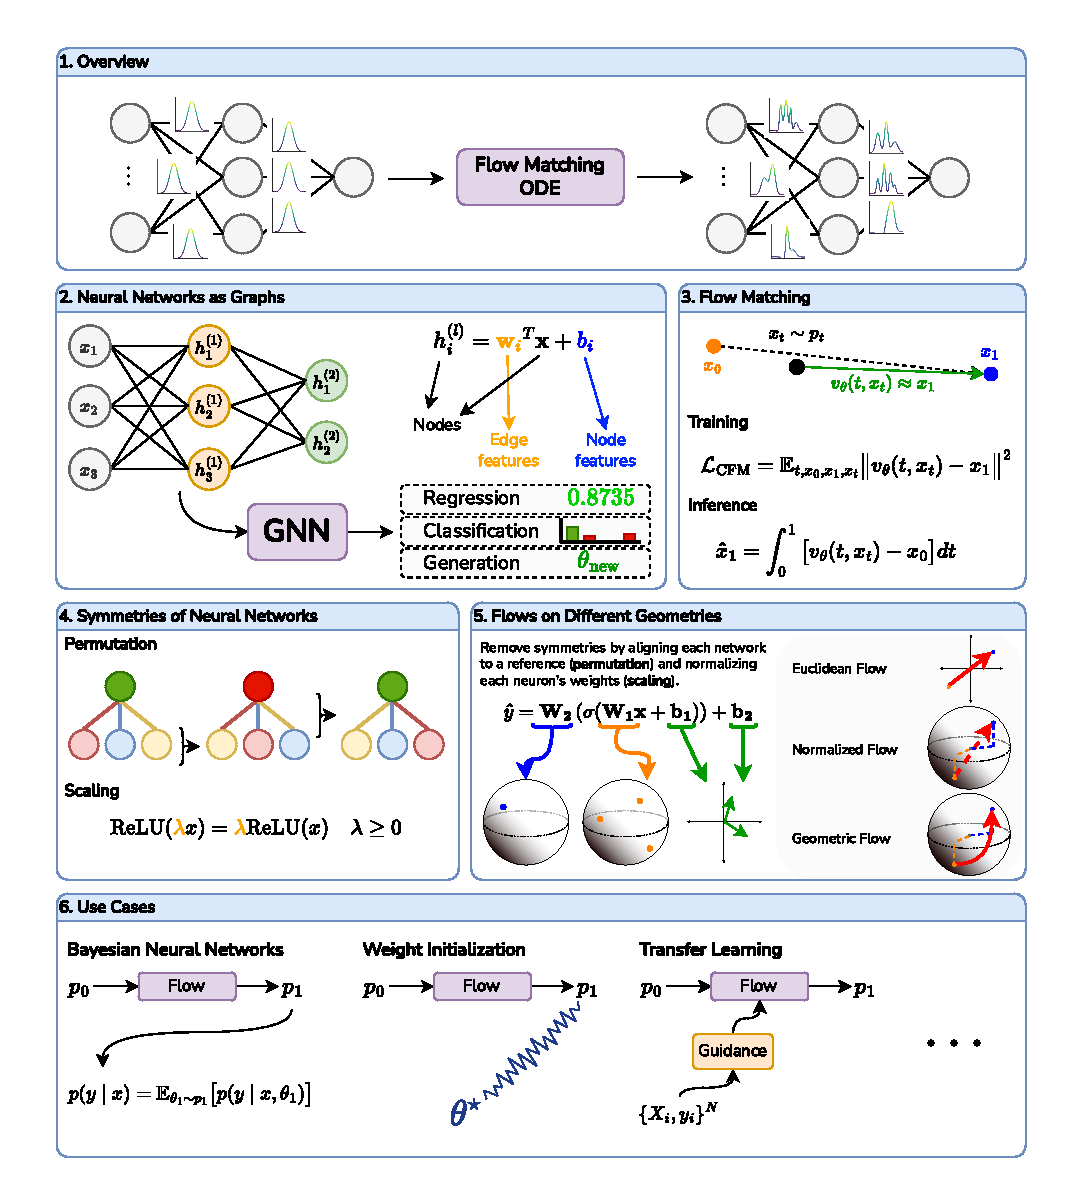
\includegraphics[width=\textwidth]{figures/weightflow.drawio.pdf}
    \caption{\label{fig:main}\textbf{Overview of our weight-space flow.} We aim to learn a flow in weight-space \textit{(1)}, modeling neural networks as graphs and processing them with GNNs \textit{(2)}, using flow matching \textit{(3)} and taking into account the symmetries of neural network weights \textit{(4)}. We propose three flows differing on how they handle this geometric structure \textit{(5)}. Potential use cases for the learned posterior include Bayesian neural networks, using it to sample initial weights, and transfer learning on new tasks through guidance during sampling \textit{(6)}.}
\end{figure}

\section{Section}
